%%%%%%%%%%%%%%%%%%%%%%%%%%%%%%%%%%%%%%%%%%%%%%%%%%%%%%%%%%%%%%%%%%%%%%%%%%

%%%%%                           Conclusion Géné                     %%%%%%
%%%%%%%%%%%%%%%%%%%%%%%%%%%%%%%%%%%%%%%%%%%%%%%%%%%%%%%%%%%%%%%%%%%%%%%%%%

\phantomsection 
\addcontentsline{toc}{chapter}{General conclusion} \mtcaddchapter
\addtocontents{toc}{\protect\addvspace{10pt}}

\vspace*{-1cm}
\begin{flushright}
\section*{\fontsize{20pt}{20pt}\selectfont\textnormal{General conclusion}}
\end{flushright}
\vspace{2cm}

\lhead[\fancyplain{}{General conclusion}]
      {\fancyplain{}{}}
\chead[\fancyplain{}{}]
      {\fancyplain{}{}}
\rhead[\fancyplain{}{}] 
      {\fancyplain{}{General conclusion}}
\lfoot[\fancyplain{}{}]
      {\fancyplain{}{}}
\cfoot[\fancyplain{}{\thepage}]
      {\fancyplain{}{\thepage}}
\rfoot[\fancyplain{}{}]
     {\fancyplain{}{\scriptsize}}

%%%%%%%%%%%%%%%%%%%%%%%%%%%%%%%%%%%%%%%%%%%%%%%%%%%%%%%%%%%%%%%%%%%%%%%%%%
%%%%%                      Start part here                          %%%%%%
%%%%%%%%%%%%%%%%%%%%%%%%%%%%%%%%%%%%%%%%%%%%%%%%%%%%%%%%%%%%%%%%%%%%%%%%%%

\section*{Outcomes}
The last few years have been very prolific for the field of markerless kinematics. Until recently, sport motion analysis had to be performed either with intrusive and complex marker-based techniques, or with rough and inaccurate markerless options. Nowadays, one can go without markers, and still obtain coherent 3D full-body joint kinematics. These methods are usually more robust than marker-based ones, and they are rapidly becoming more and more accurate. Our decision of crafting a robust triangulation procedure, and of constraining rough 3D coordinates to a biomechanically consistent skeletal model, makes it almost as accurate as marker-based solutions, at least for walking, running, and cycling tasks. Such an approach has been proven to also work with on-field sports constraints, such as the use lightweight, wireless, consumer-grade cameras, which are not straightforward to calibrate and synchronize. Equipment can also be detected along with the athlete, although much like with marker-based techniques, it is not yet conclusive in case closed-loop constraints are enforced. Both in boxing and in BMX racing, key performance indicators could be retrieved satisfyingly. 

The Pose2Sim workflow we proposed aimed at building a bridge between the computer vision and biomechanics communities, by using two of the most renown tools of their respective fields: OpenPose for 2D pose estimation, and OpenSim for 3D joint kinematics. This tool is open-source, versatile, and accessible to sports scientists rather than to computer vision specialists. As it was made to be useful and usable, it is also used: the University of Bath is currently creating a GUI around it, a (non-free) Blender add-on which integrates it has been released, and the GitHub repository is active. It has also been quoted by the University of Stanford, which later developed their own 3D markerless solution \cite{Uhlrich2022}. 

% \vskip 0.4cm

\section*{Limits and perspectives}
Some challenges remain, which would determine the adoption of markerless kinematic tools by the community of sports science. According to the most reported GitHub issues on Pose2Sim, the main stumbling block for users is calibration. Hence, there is definitively a need for an easier procedure, such as the one proposed by \cite{Argus}, or even an auto-calibration method based on known limb sizes seen across multiple views. As we have demonstrated, an imperfect calibration does not degrade results much after 3D reconstruction and skeletal model constraints have been applied. Moreover, the feedback given to athletes and coaches should be provided quickly enough for them to integrate it, and adjust their motion patterns before their next trial sequence. Quasi-real-time can be achieved which research-grade cameras, as videos are directly downloaded after each sequence on the master computer, which can run Pose2Sim in the background. For wireless consumer-grade cameras, it is more complicated, although some devices can sometimes remotely control the media downloading. Additionally, by essence, team sports are practiced as a group, and thus performing multi-person inverse kinematics can be important. Although we did not implement it yet, we described methods to achieve it. Finally, sports scientists are usually more at ease with graphical user interfaces than with command line, and coaches prefer a visual feedback rather than joint angle waveforms. A tool for visualization in Maya has been developed, but it is not yet ready for release. Moreover, as all the tools used and proposed here are open-source, it would make more sense to propose it as a standalone software application, or as a free Blender add-on (see Figure~\ref{fig_blendermocap} for its planned features, and Figure~\ref{fig_mayamocap} for the features already developed on the Maya-MoCap toolbox). Furthermore, this work gave rise to a projected collaboration with the University of Bath, which is currently developing a GUI for Pose2Sim, and with whom we plan to build a new sports dataset for more accurate markerless kinematics. 

% \vskip 0.4cm

\section*{Future prospects}
Current datasets for 2D pose estimation are not accurately labelled, they suffer from a dearth of keypoints, and they are not trained to recognize sports poses nor any equipment. Building a whole new dataset could solve these issues.

Note that it should not base its labeling on marker positions, that could be interpreted as visual cues, which are not available in real sports situations. However, this condition is not sufficient: the dataset should also be large and diverse enough, represent a wide variety of body types and of sports movements \cite{Seethapathi2019}, and include images with motion blur such as found in sports videos. One way to do it is to build a synthetic dataset. For example, a mass of c3D motion files could be gathered from various sports, and be used to fit an SMPL+H mesh \cite{Pavlakos2019} with AMASS \cite{Mahmood2019}. These data could be augmented with already existing datasets for daily life activities, such as Agora \cite{Patel2021}. Then, it would be possible to take advantage of the fact that the topology of an SMPL mesh is constant, and assume that only labelling the first frame of any given sequence should be sufficient: label positions should be consistently propagated to the next frames. At this stage, one could place as many virtual markers as needed, for a precise evaluation of any movement and pose. However, only an expert should perform this task, and make sure that markers are correctly positioned: crowd-sourcing this task, like it is done for more basic image classification and segmentation with ImageNet \cite{Deng2009}, has been proved to lead to systematic offset errors \cite{Needham2021b}. Finally, random clothing, background, and light could be added (see \cite{Wood2021,Bolanos2021} for a detailed workflow), as well as variations in SMPL shape parameters. The scene would be filmed with numerous virtual cameras, in order to gather a large amount of diverse perspectives, and virtual markers would be automatically projected on the camera planes. 

This would result in an extensive sports dataset, created with minimal labelling work, on a potentially infinite amount of views. Nevertheless, before training the network, one should make sure that the generated data is as diverse as the real world, by using one of the metrics proposed by \cite{Borji2019, Borji2022}. Additionally, keypoint positions need to be precise enough: SMPL shape vertices can sometimes be more than 5 cm apart, which could cause imprecision errors similar to skin artifacts. Besides, instead of constraining pose estimation results with a physically consistent skeletal model, it would be interesting to develop a physics-informed pose estimation model \cite{Raissi2019,Xu2020a}, which would offer the opportunity of embedding the kinematics priors as early as possible in the learning process, or conversely as a refinement step upon triangulation \cite{Hua2022}.


\begin{figure}[hbtp]
      \centering
      \Rotatebox{90}{
      \def\svgwidth{1\columnwidth}
      \fontsize{10pt}{10pt}\selectfont
      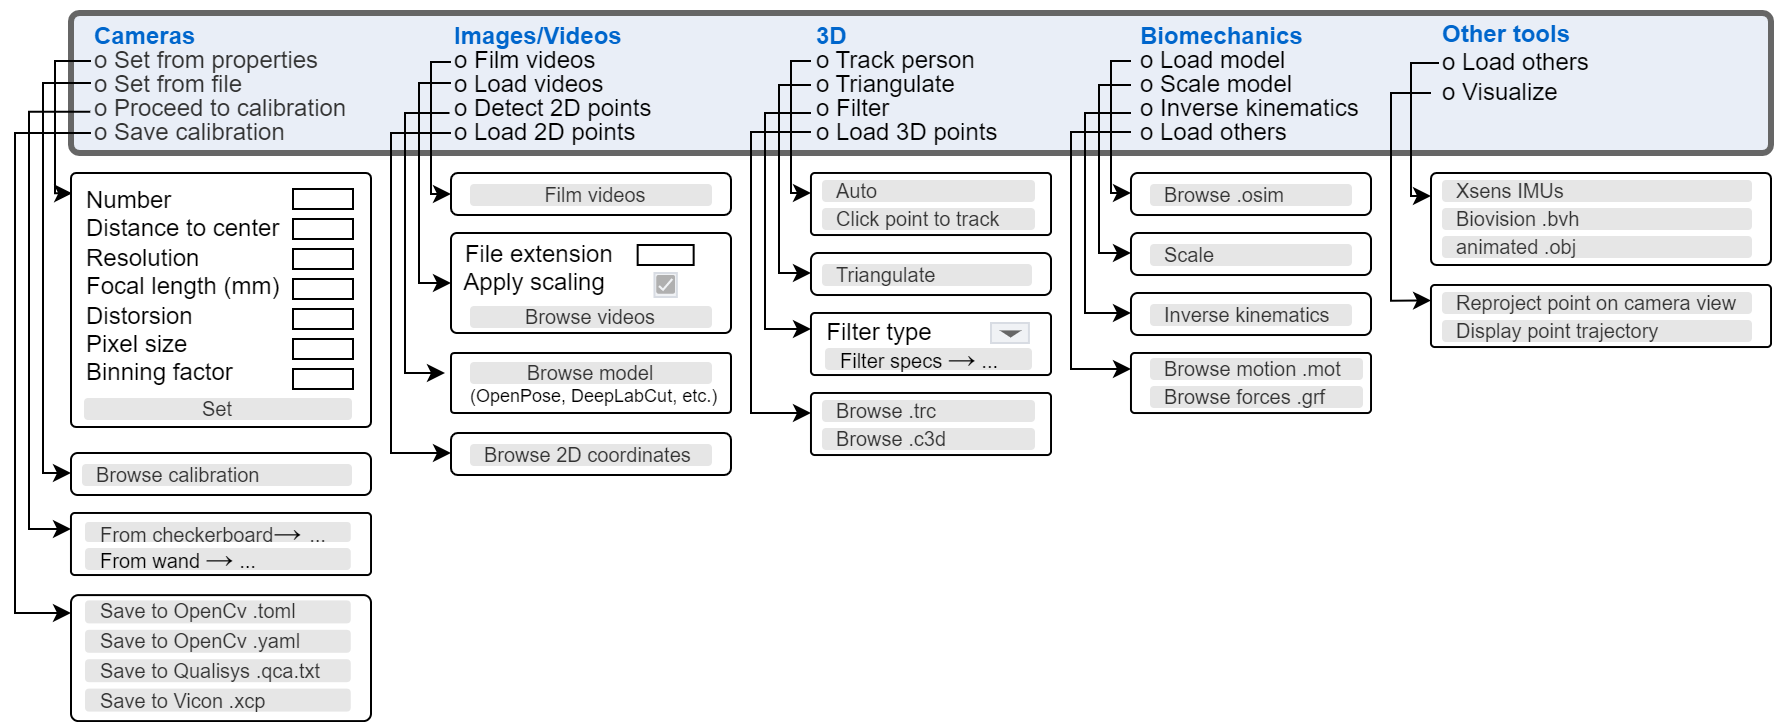
\includegraphics[height=0.6\linewidth]{"../Chap3/Figures/Fig_MayaMocap3.png"}}
      \caption{Planned features of the future Blender add-on. See Figure~\ref{fig_mayamocap} for reference to the already developed Maya-Mocap add-on.}
      \label{fig_blendermocap}
\end{figure}




% marche course vélo bmx boxe chill nage danse (lancer, parkour?)